\section{Zweite Evaluation}
\subsection{Morphologischer Kasten}
In der ersten Phase der zweiten Evaluation haben wir die Ergebnisse der ersten Evaluation in einem morphologischen Kasten zusammengefasst. Mithilfe dieses morphologischen Kastens haben wir drei mögliche Lösungskonzepte zusammengestellt. Hierbei haben wir uns an der Teilfunktion Treppensteigen orientiert. Von da aus haben wir die restlichen Komponenten hinzugefügt. Die Hauptunterschiede unserer drei möglichen Lösungskonzepte (Frosch, 3-teiliger Hebemechanismus, Beine) liegen bei den Teilfunktionen Treppensteigen, Lenkung und Fortbewegung.

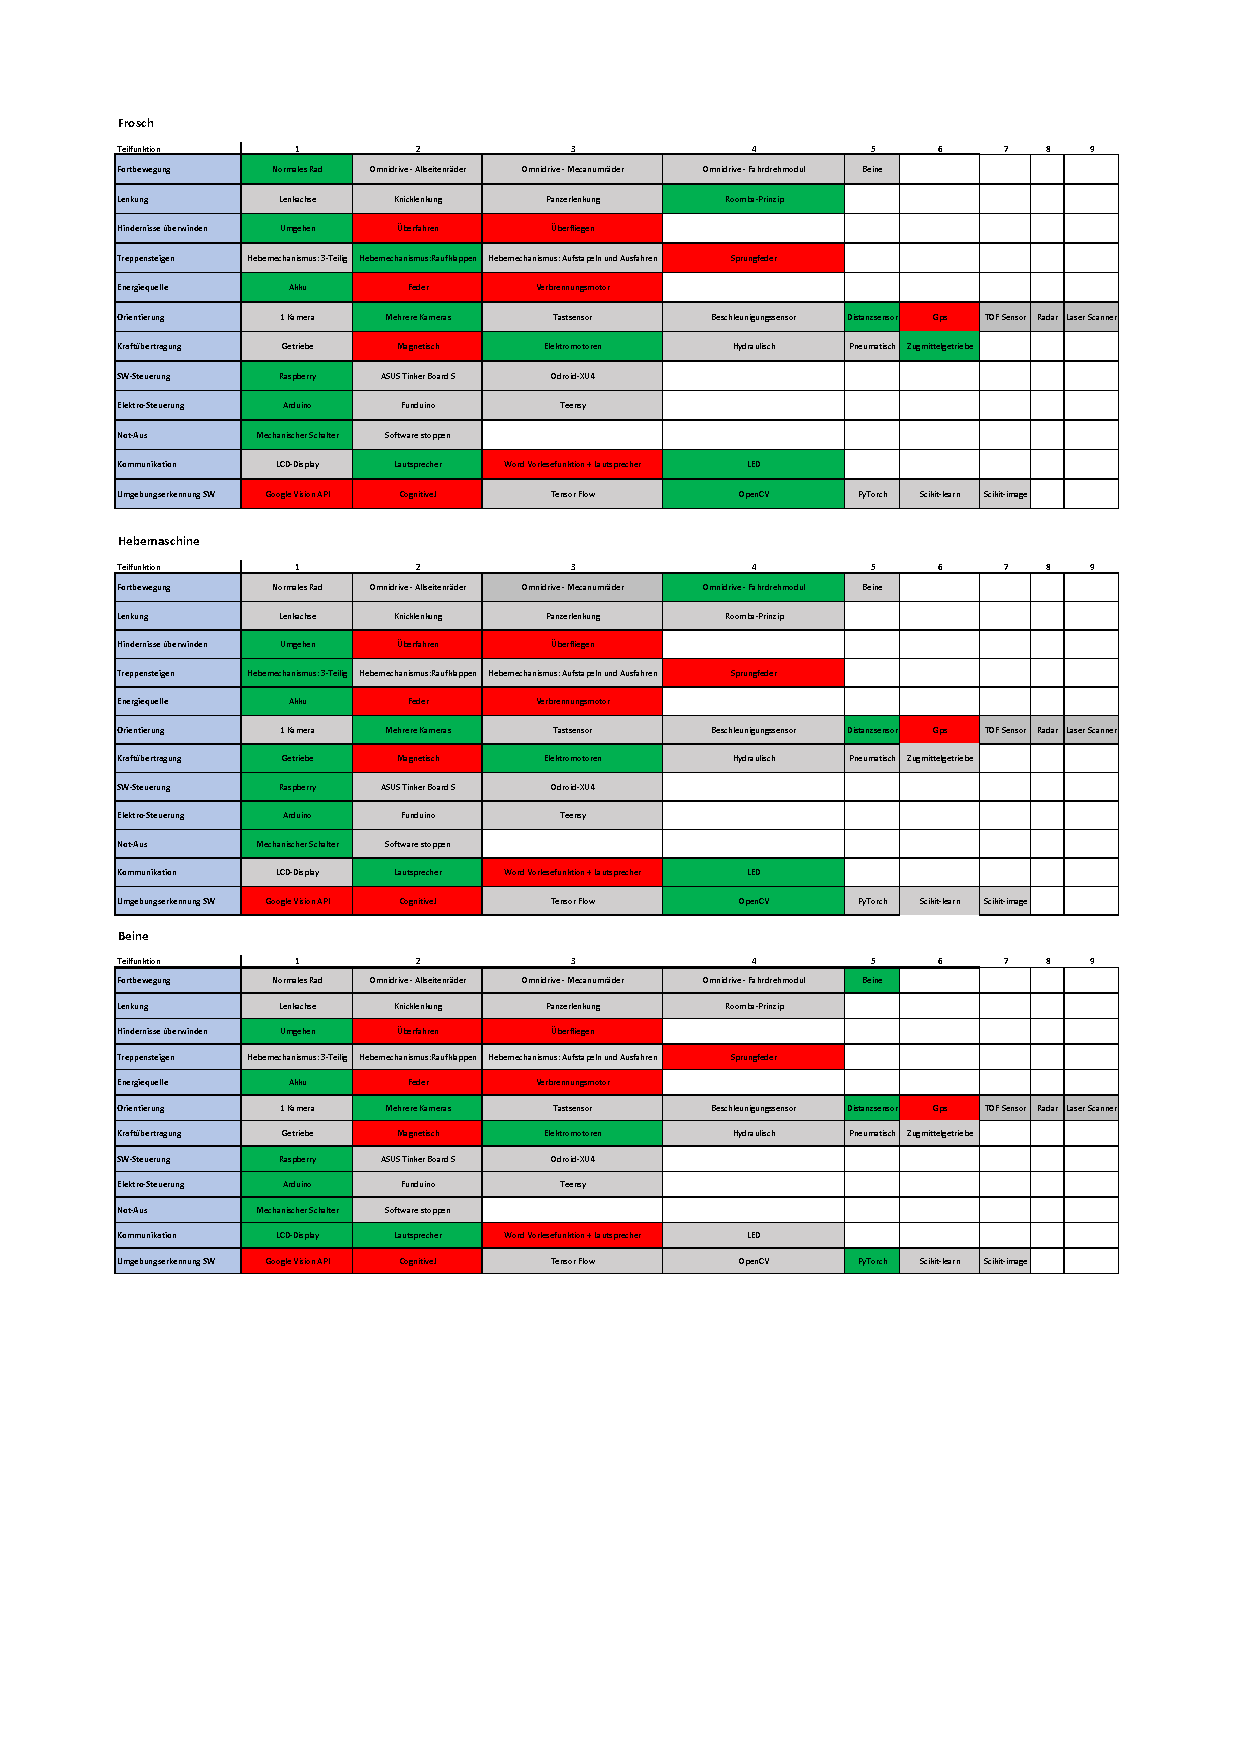
\includepdf[
  pages={1-},
  scale=1,
  pagecommand={\pagestyle{fancy}}
]{assets/MorphologischerKasten.pdf}

\subsection{Nutzwertanalyse}
In der zweiten Phase haben wir die drei möglichen Lösungskonzepte anhand einer Nutzwertanalyse einander gegenübergestellt. Wichtige Kriterien waren hierbei z.B. der Entwicklungsaufand, die Zuverlässigkeit, die Geschwindigkeit, die Kosten. 

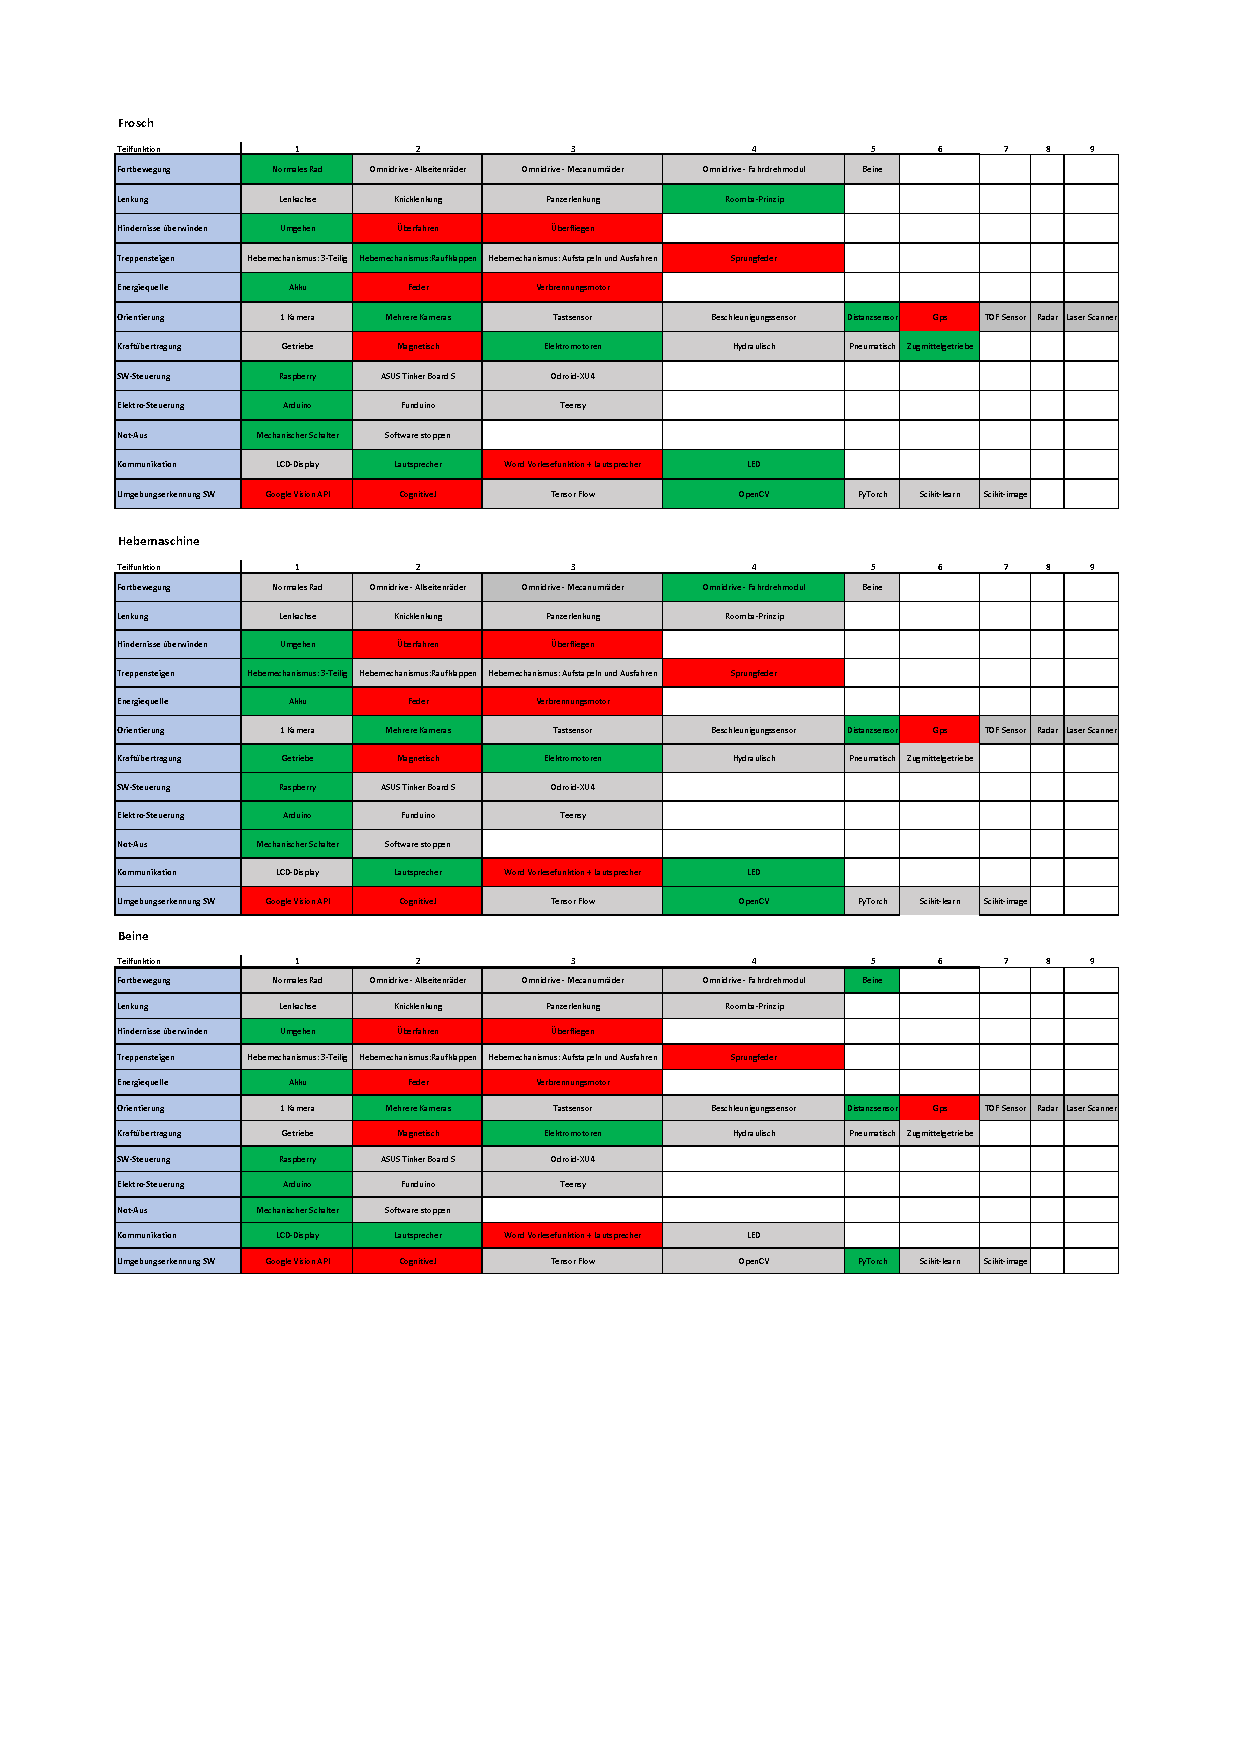
\includepdf[
  pages={1-},
  scale=1,
  pagecommand={\pagestyle{fancy}}
]{assets/MorphologischerKasten.pdf}